% roboto, callout, [[speech bubble]], sans, [[append after command]], sfdefault, arc, [[block diagram]]
\PassOptionsToPackage{usenames,dvipsnames}{xcolor}
\documentclass[tikz,border=2]{standalone}
\usetikzlibrary{shadows,arrows,shapes,positioning,calc,backgrounds,fit,automata}
%
%%%%%%%%%%%%%%%%%%%%%%%%%%%%%%%%%%%%
%% Common preamble
%%%%%%%%%%%%%%%%%%%%%%%%%%%%%%%%%%%%
% PAGE
%% \usepackage{fullpage}
% FONTS
%%\usepackage{lmodern} % enhanced version of computer modern
\usepackage[sfdefault]{noto}
\usepackage[T1]{fontenc} % for hyphenated characters
%% \usepackage{gillius2}
%% \renewcommand{\familydefault}{\sfdefault}
\usepackage{amssymb} % for \checkmark
\usepackage{mathtools} % contains amsmath which comes with align
\usepackage{amsthm}
%%\usepackage{enumitem}
\usepackage{microtype} % some compression
%%%%%%%%%%%%%%%%%%%%%%%%%%%%%%%%%%%%
\usepackage{subfig}
\usepackage{tikz}
\usetikzlibrary{spy,shadows,arrows,shapes,positioning,calc,backgrounds,fit,automata}
\newcommand{\score}{\text{score}}

\definecolor{Green}{HTML}{BCD695}
\definecolor{Darkgreen}{HTML}{0092A0}
\definecolor{Darkbrown}{HTML}{474342}
\definecolor{Brown}{HTML}{6C6B67}
\definecolor{Lightbrown}{HTML}{A3A5A6}
\definecolor{Lighterbrown}{HTML}{E0DCDB}


\newcommand{\dunder}[1]{\underline{\underline{#1}}}
\newcommand{\dmax}{d_{\max}}
\newcommand{\cost}{\text{cost}}
%\newcommand{\comment}[1]{{\color{red}#1}}
\newcommand{\wmin}{w_{\min}}
\newcommand{\copt}{C_{\text{OPT}}}
\newcommand{\TikZ}{Ti\textit{k}Z\xspace}
\newcommand{\tuta}{\emph{T. absoluta}}
\newcommand{\prempt}{\textsc{PREMpT}}
\newcommand{\parnode}[1]{\parbox{3cm}{\centering #1}}

%%
%% This ``scales'' the font. Don't extend too much beyond 128x96
%% Uncomment the next line for default sizes:
%% \setbeamercolor{block title}{use=structure,fg=white,bg=black!75!white}
%% \setbeamercolor{block body}{use=structure,fg=black,bg=black!10!white}
%
%% ----------------------------------------------------------------------
%%
\begin{document}
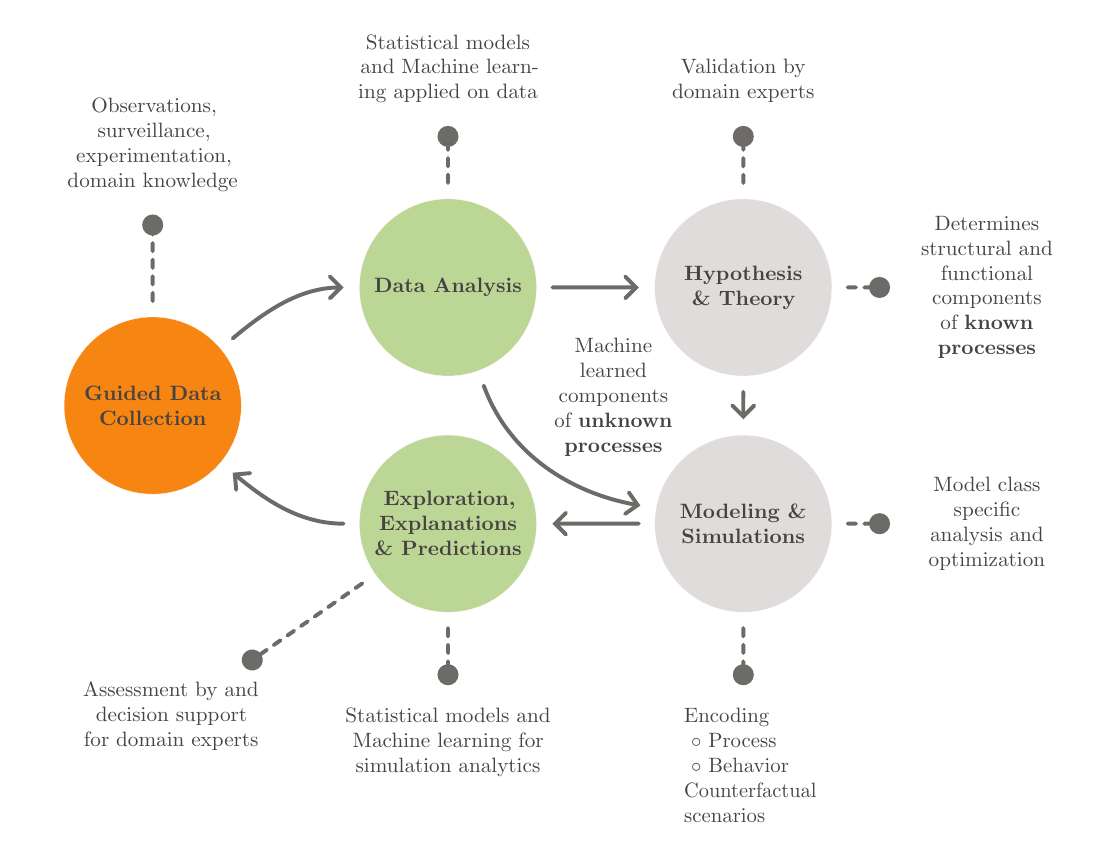
\begin{tikzpicture}
[scale=.75,auto,transform shape,
    edge/.style={line cap=round,Brown,>=angle 90, shorten >=2mm, shorten <=2mm, line
    width=.5mm},
every node/.style={text=Darkbrown},
explain/.style={align=center,text width=3cm,text=Darkbrown},
callout/.style={align=center,font=\bfseries,text
width=2cm,fill=Brown,text=white,ellipse callout},
block/.style={font=\bfseries,text width=2.5cm,circle,align=center,minimum width=3cm,inner sep=0mm,draw=white,ultra thin,fill=Green, append after
command={\pgfextra{\node[fill=none,circle,inner sep=-3mm,thick,fit=(\tikzlastnode)]{};}}},
dedge/.style={line cap=round,line width=.5mm,shorten >=2mm, shorten
<=2mm,Brown,dashed}]

\def\ushift{2}

\node[block,fill=BurntOrange] (data) {Guided Data Collection};
\node[explain,anchor=south,above=of data,shift={(0,)},text width=4cm] (edata) {
    Observations, \\
    surveillance,  \\
    experimentation, \\
    domain knowledge};

\node[block] (ana) at (5,\ushift) {Data Analysis};
\node[explain,anchor=south,above=of ana,shift={(0,.5)},text width=4cm] (eana) {
    Statistical models and 
    Machine learning applied on data
    };

\node[block,fill=Lighterbrown] (hyp) at (10,\ushift) {Hypothesis \& Theory};
\node[explain,anchor=south,above=of hyp,shift={(0,.5)},text width=4cm] (ehyp) {
    Validation by \\ domain experts
    };
    \node[explain,anchor=west,right=of hyp,shift={(.25,0)},text width=2.5cm]
(ehyp1) {
    Determines structural and functional components of {\bf known
    processes}
    };

\node[block,fill=Lighterbrown] (sim) at (10,-\ushift) {Modeling \& Simulations};
\node[explain,anchor=north,align=left,below=of sim,shift={(0,-.5)},text width=2cm] (esim) {
    Encoding \\
    ~$\circ$ Process \\
    ~$\circ$ Behavior \\
    Counterfactual scenarios
    };
    \node[explain,anchor=west,right=of sim,shift={(.25,0)},text width=2.5cm]
(esim1) {
    Model class specific analysis and optimization
    };


\node[block] (sana) at (5,-\ushift) {Exploration, Explanations \& Predictions
};
\node[explain,anchor=north,below=of sana,shift={(0,-.5)},text
width=4cm] (esana) {
    Statistical models and Machine learning for simulation analytics
    };
    \node[explain,anchor=north,below left=of sana,shift={(-.5,-.5)},text
width=4cm] (esana1) {
    Assessment by and decision support for domain experts
    };

\draw[dedge,-*] (data) -- (edata);
\draw[dedge,-*] (ana) -- (eana);
\draw[dedge,-*] (hyp) -- (ehyp);
\draw[dedge,-*] (hyp) -- (ehyp1);
\draw[dedge,-*] (sim) -- (esim);
\draw[dedge,-*] (sim) -- (esim1);
\draw[dedge,-*] (sana) -- (esana);
\draw[dedge,-*] (sana) -- (esana1);


\draw (data) edge[edge,->,out=40,in=180] (ana);
\draw (ana) edge[edge,->,out=0,in=180] (hyp);
\draw (hyp) edge[edge,->,out=-90,in=90] (sim);
\draw (sim) edge[edge,->,out=-180,in=0] (sana);
\draw (sana) edge[edge,->,out=-180,in=-40] (data);
\draw (ana) edge[edge,->,out=-70,in=170] node [explain,text width=2cm]
{Machine learned components of {\bf unknown processes}} (sim);

\end{tikzpicture}
\end{document}

